\chapter{Analyse \& Design ( 25 \%)}
\label{chap:design}

\section{Grundlegende Systemarchitektur}


\begin{figure}[ht] 
  \label{fig:grob-layout-komponenten}
  \begin{center}
      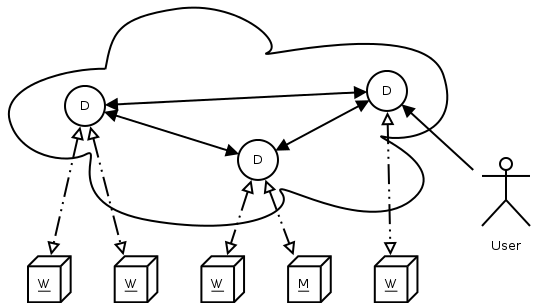
\includegraphics[width=\textwidth]{imageinput/grob-layout-komponenten.png}
  \end{center}
  \caption{\"Ubersicht uber Systemkomponenten - physisch}
\end{figure}


\begin{figure}[ht]
  \label{fig:grob-layout-komponenten-logisch}
  \begin{center}
      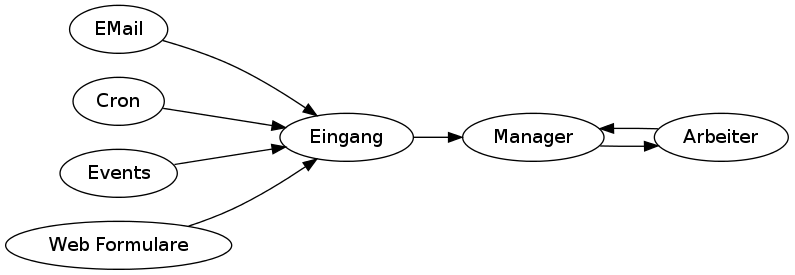
\includegraphics[width=\textwidth]{imageinput/grob-layout-komponenten-logisch.png}
  \end{center}
  \caption{\"Ubersicht ber Systemkomponenten - logisch}
\end{figure}


\section{Grundlegendes Datenschema}


\begin{figure}[ht] 
  \label{fig:datenstrukturen}
  \begin{center}
      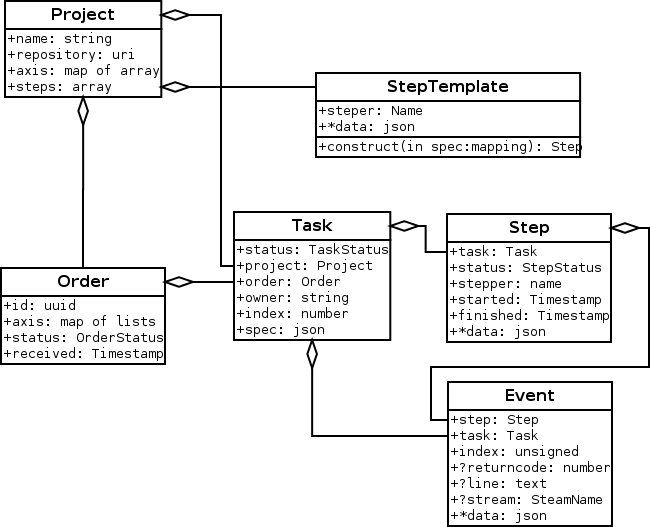
\includegraphics[width=\textwidth]{imageinput/datenstrukturen-step-templates.png}
  \end{center}
  \caption{Grundlegende Datenstrukturen}
\end{figure}




\section{Grundlegende Logik der Komponenten} %XXX: bettern na

% below here - unterordnen logik`

\subsection{Vorbereitende Primitiven}

\subsubsection{listen\_changes}
\subsubsection{watch\_for}
\subsubsection{gather\_next}
\subsubsection{run\_callbacks}


\subsection{Auftragsannahme}


\begin{figure}[ht] 
  \label{fig:lebenszyklus-auftrag-eingang}
  \begin{center}
      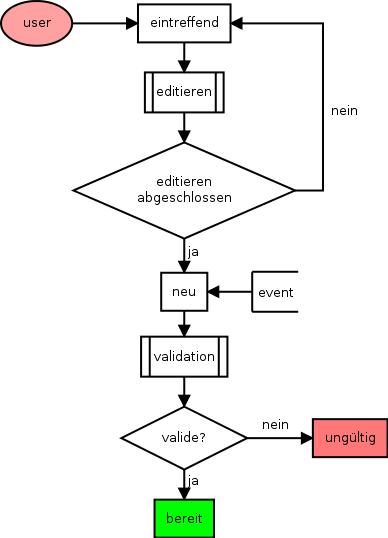
\includegraphics[height=5in]{imageinput/lebenszyklus-auftrag-eingang.png}
  \end{center}
  \caption{Auftragsannahme: Flowgraph}
\end{figure}

- 2 teile
- eingang \& validation


\subsubsection{Eingang}

\begin{verbatim}
- quellen
- editiern
- typisches
\end{verbatim}

\subsubsection{Validation}
\begin{verbatim}
- notwendig weil ...
- beispiele fuer checks
- theoretisch
\end{verbatim}


\subsection{Management}

\begin{figure}[ht] 
  \label{fig:lebenszyklus-auftrag-abarbeitung}
  \begin{center}
      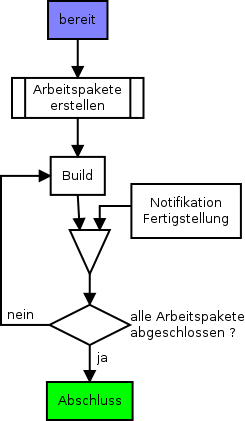
\includegraphics[height=4in]{imageinput/lebenszyklus-auftrag-abarbeitung.png}
  \end{center}
  \caption{Auftragsannahme: Flowgraph}
\end{figure}

\subsubsection{Auftragsvorbereitung}

\begin{verbatim}
- 
\end{verbatim}


\subsubsection{Bereitstellung von Arbeitspacketen}
\subsubsection{Abschluss von Auftr\"agen}


\subsection{Zuteilung/Abarbeitung von Arbeitspacketen}


\subsubsection{Lebenszyklus eines Arbeitspacketes}


\begin{figure}[ht] 
  \label{fig:lebenszyklus-arbeitspaket}
  \begin{center}
      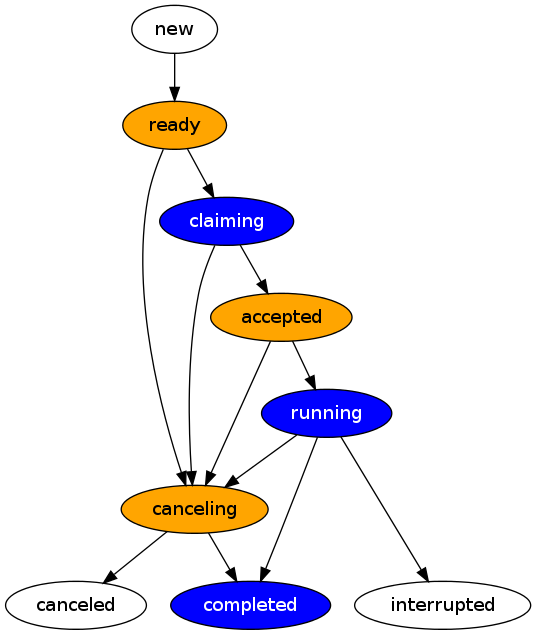
\includegraphics[height=4in]{imageinput/lebenszyklus-arbeitspaket.png}
  \end{center}
  \caption{Lebenszyklus eines Arbeitspacketes bei Ausschreibungen}
\end{figure}


\subsubsection{Vorbereitung Abarbeitung}

\subsection{\"Uberblick Zuteilungsmethoden}


\begin{verbatim}
- diese sektion besch. sich mit


- methoden
    - token basiert
    - ausschreibungsbasiert

\end{verbatim}


\subsubsection{token basierte zuweisung}

\begin{verbatim}
- arbeiter teilen nur mit, dass sie arbeitsfaehig sind
- manager kontrolliert wer welchen auftrag erhaelt
cons:
    - fuer erweiterte use-cases extra wissen im manager notwendig
\end{verbatim}

\begin{figure}[ht] 
  \label{fig:auftrag-zuteilung-token}
  \begin{sequencediagram}
      \newinst{worker}{:Worker}
      \newinst[1]{manager}{:Manager}
      \mess{worker}{token <spec>}{manager}
      \mess{manager}{work <spec>}{worker}
      \mess{worker}{result}{manager}
  \end{sequencediagram}
  \caption{Auftragszuteilung: Tokenbasiert}
\end{figure}

\subsubsection{ausschreibungsbasierte zuweisung}

\begin{verbatim}
- manager teilt offene auftraegeposten mit (in datenbank verf.)
- arbeiter konkurieren um offene auftraege
- manager entscheidet wer den aufrag dann erhaelt


- autonomere arbeiter
- manager muss nur noch entscheiden wer, nicht mehr warum
- aufgrund der datenbank konzeptuell einfacher -> beweis oder weg
\end{verbatim}

\begin{figure}[ht] 
  \label{fig:auftrag-zuteilung-claim}
  \begin{sequencediagram}
      \newinst{workera}{:Worker A}
      \newinst[1]{manager}{:Manager}
      \newinst[1]{workerb}{:Worker B}
      \mess[1]{manager}{availiable}{workera}
      \prelevel
      \prelevel
      \mess[1]{manager}{availiable}{workerb}

      \mess[1]{workera}{claim}{manager}
      \prelevel
      \prelevel
      \mess[2]{workerb}{claim}{manager}
      %XXX: better call?
      %\prelevel
      %\prelevel
      %\begin{call}{manager}{approve}{manager}{workera}
      %\end{call}
      \mess{manager}{approve A}{workera}
      \prelevel
      \mess{manager}{approve A}{workerb}
  \end{sequencediagram}
  \caption{Auftragszuteilung: Ausschreibungsbasiert}
\end{figure}


\subsubsection{Abschluss Abarbeitung}

- ende der arbeisschritte
- zusammenfassung resultat
- endscheidung fehlschlag oder nucht


\subsection{Abarbeitung von Arbeitspacketen}

\begin{verbatim}
- lineare abarbeitung
- abbrich bei fehlschlag
\end{verbatim}

\subsubsection{Arbeitsschritte}


\begin{figure}[ht] 
  \label{fig:lebenszyklus-arbeitsschritt}
  \begin{center}
      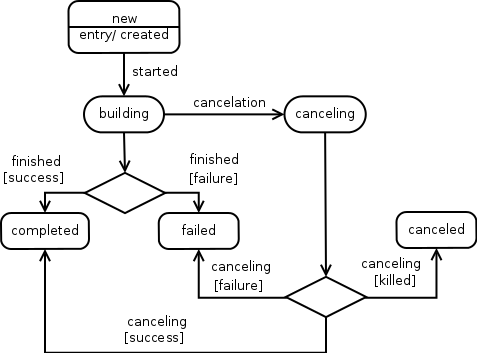
\includegraphics[height=3.4in]{imageinput/lebenszyklus-arbeitsschritt.png}
  \end{center}
  \caption{Stategraph eines Arbeitschrittes}
\end{figure}

\begin{verbatim}
- kill wird in der impl nicht betrachtet

\end{verbatim}


\subsubsection{Datensammlung zur Laufzeit}

\begin{verbatim}
- sinn/echtzeit?

- beispielhaft
    - STDOUT/ERR
    - exakte testresultate/reports
\end{verbatim}

\subsubsection{Datensammling nach Abschluss eines Schrittes}

- junitxml
- logfiles

- betrachtung extra schritt vs interne funktion

\subsubsection{Abschluss von Arbeitschritten}

- returncodes
- fehler

\subsection{Arten von Arbeitschritten}

\subsubsection{\"Ubersicht}

\begin{figure}[ht] 
  \label{fig:klassen-arten-arbeitsschritt}
  \begin{center}
      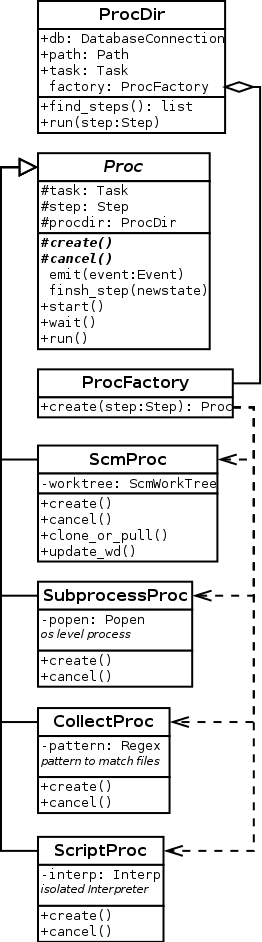
\includegraphics[height=3.5in]{imageinput/klassen-arten-arbeitsschritt.png}
  \end{center}
  \caption{Arten von Arbeitschritten}
\end{figure}



\subsubsection{Prozessaktionen}

- was/wozu
- datensammlung laufzeit
- datensammlung ende

\subsubsection{Quellcode Management Aktionen}

- ablauf, beispiele



\section{Besondere Ans\"atze zur Datenbankinteraktion}

%XXX: http://dbmsmusings.blogspot.de/2010/04/problems-with-cap-and-yahoos-little.html


\subsection{CAP Abdeckung}

\begin{verbatim}
- ``2 of 3''
- verschiedene aspekte der applikation haben unterschiedliche anforderungen
- 

\end{verbatim}


% http://www.infoq.com/articles/cap-twelve-years-later-how-the-rules-have-changed

\begin{verbatim}
- wie ber in cap \ref{sec:basic:cap}

\end{verbatim}

\subsection{statusmaschienen zur konsistenzwahrung}

\begin{verbatim}
- konzept der knuepfung von transitionen an operatoren,
  - so gestalten, das auch bei partitionierung inkonsistenzen durch die konsistenzbedingungen der statusmaschienen unmoeglich sind

\end{verbatim}



\section{Logisches Gesammtkonzept}



\section{Benutzerinterface}

% kann krit
% kein tolles
% nur werkzeuge


\section{zusammenfassung}

was kommt
was kommt nicht
